%% simulationSoftware.tex
%%

%% ==============
\chapter{Simulation of muon induced background}
\label{ch:Simulation of muon induced background}
%% ==============
  To compare the data aquired to theoretically expected values, a Geant4 simulation of cosmic showers has been set up including the geometry of the main spectrometer as well as the muon modules. Using this software, any number of inciding muons can be simulated and the effect on the main spectrometer and the muon modules can be evaluated. It was especially relevant to achieve estimations on which amount of the muons travelling through the main spectrometer would be registered by the muon modules. This would then make it possible to estimate the overall rate and probabilities for muons inciding to also induce electrons etering the spectrometer.
  %% ===========================
  \section{Geant4}
  \label{ch:Simulation software:sec:Geant4}
  %% ===========================
  The Geant4 package is a powerful tool for simulation of particles. It has loads of possible interactions already integrated making it easy for the user to set up and run simulations. After setting up geometry and detectors, the user starts a run. Each run may consist of one or more events. During a single run, a loop of processes is called:
  \begin{itemize}	
  	\item Primary Generator Action
  	\item Run action
  	\item Event action
  	\item Stacking action
  	\item Tracking action
  	\item Stepping action
  \end{itemize}
  Of course inside each run usually there are many event actions and inside every event action, there are multiple tracking actions.
  For user interaction, for each item above, classes with the addition 'user' to the base classes name can be called before or after the standard action class. An example is the class G4UserEventAction invoked before and after each call of G4TrackingAction. It contains two member classes, namely BeginOfEventAction and EndOfEventAction that let the user decide what to do at this point. Through those, it is possible to change behaviour of the simulation or extract data needed. In this case, for every event, if more than one module has been hit, the copy numbers of those are pushed back to a vector of event data.  
  Running the simulation, one can either interactively enter commands or write those to a .mac file, by default the vis.mac file, which are then sequentially executed.
  


  %% ===========================
  \section{Geometry setup}
  \label{ch:Simulation software:sec:Geometry setup}
  %% ===========================
  To set up a geometry, the class G4VUserDetectorConstruction is used. B1DetectorConstruction inherits from that as a base class and additionally contains all of the geometrical parameters needed for the setup such as radii of the main spectrometer cones or positions and extent of the muon modules. Every shape generated is made up of both a logical volume G4LogicalVolume and a physical volume G4PhysicalVolume. The logical volume describes the intrinsic properties of the geometric object added: its shape, its size and its material. The physical volume accepts a logical volume as input providing position and alignment of the previously defined.
  Inside the detector construction class, all of the materials used in the simulation need to be defined as well. These are the components of the air outside and inside the spectrometer including pressures and constitution, the stainless steel of the spectrometer wall and the scintillator material of the muon modules.
  The main spectrometer geometry was already \todo{written by who?} existent but had to be modified as many border volumes were implemented. These were very flat volumes covering any area of the main spectrometer not needed for this simulation. Additionally, the muon modules have been added as sensitive volume. Keeping in mind that one wants to not only distinguish whether a module has been hit, but also which one. That is why the logical volume for every module is the same whereas the physical volume is a copy of the first at different world coordinates making them identifiable via their individual copy number.
  
  \begin{figure}
  	\centering
  	\includegraphics[width = \textwidth]{graphics/simulation/geometrySetup.eps}
  	\caption[Simulation geometry setup]{The image shows a screenshot of the geometry setup as displayed in the openGL viewer. The three groups of muon modules are visible right below the large main spectrometer structure. In addition, two incident muons are displayed together with secondary particles they generated.}
  \end{figure}

  
  %% ===========================
  \section{Muon generator}
  \label{ch:Simulation software:sec:Muon generator}
  %% ===========================  
  
  Muon generation was realized through the primary generator action. The angular distribution suggested by Henrik Arlinghaus \cite{DTArlinghaus} was implemented. The angular rate dependence is shown in \ref{fig:rateDependance}.The energy was set to \todo{reasonable value} disregarding the actual energy distribution as this was mainly about flight paths that are not strongly dependent on energy at high energies. Starting positions were spherically distributed, with the direction towards the origin, which is in the center of the main spectrometer. Positions were then randomly moved in a volume surrounding the spectrometer to account for the non-point like structure of the detection system as a whole, while the distribution describes a single point in space.
  \begin{figure}
  \centering
  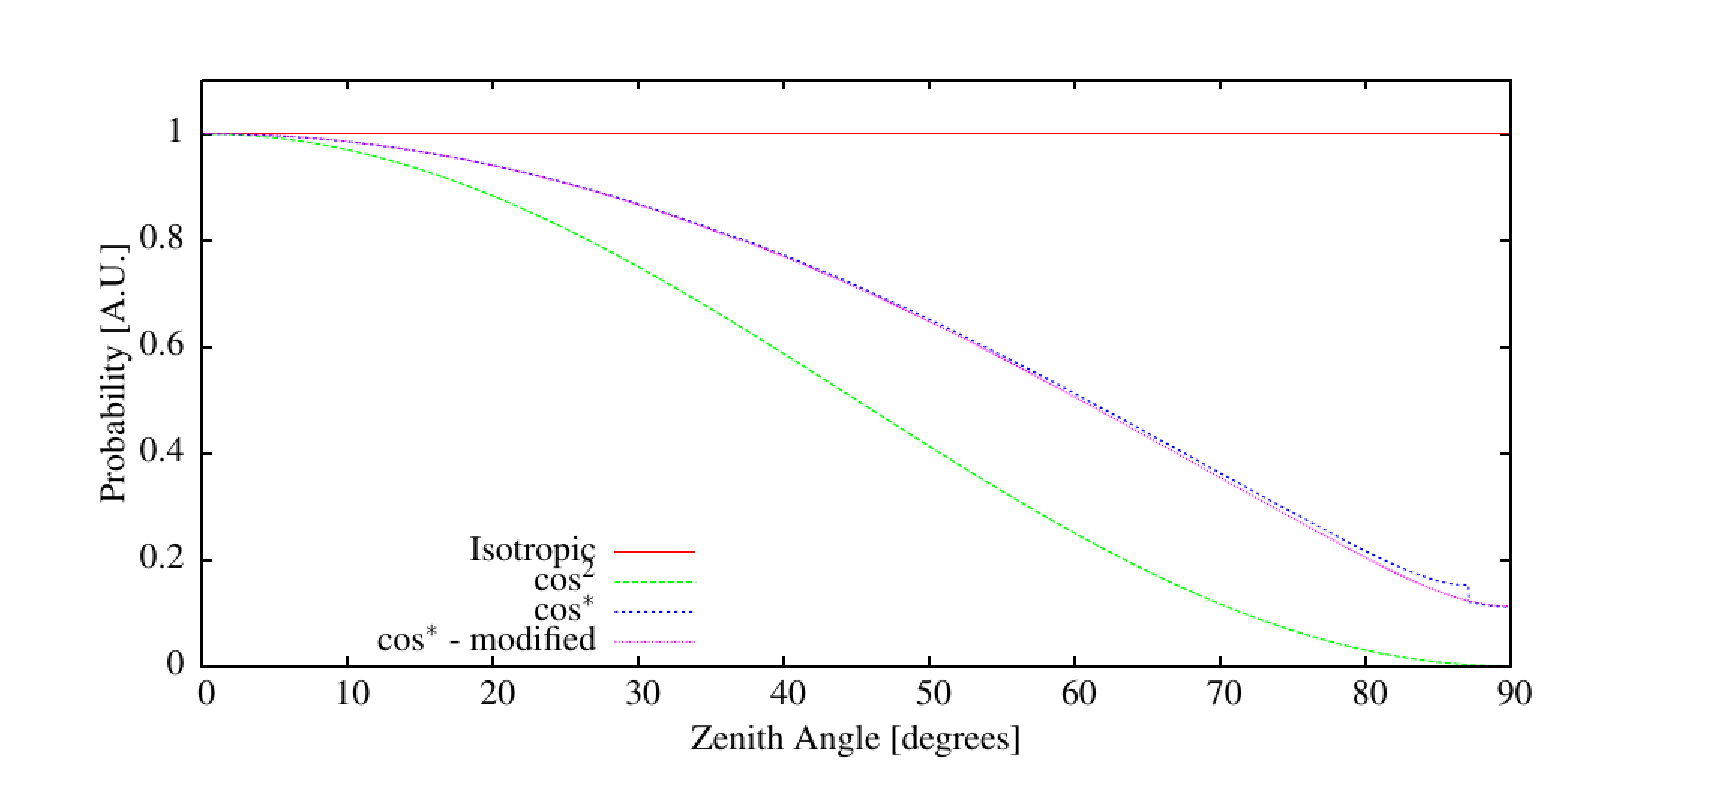
\includegraphics[width = 0.8\textwidth]{graphics/simulation/angularDistributions.eps}
  	\caption[Muon rate dependance on zenith angle]{Different distributions of }
  	\label{fig:rateDependance}
  \end{figure}
  The distribution used is the cos* distribution.
  \begin{equation}
  	\cos^*{\left(\theta \right)} = S(\Theta)\cos^{**}{\left(\theta\right)}
  \end{equation}
  with
  \begin{equation}
  	S(\theta) = 0.986 + 0.0007\sec{\theta}
  \end{equation}
  and $S(\theta)$ described by a polynomial
  \begin{equation}
  	\sum_{i=0}^{4}{c_i \cos^i{\theta}}.
  	\label{eq:coeffs}
  \end{equation}
  The coefficients are defined differently for different angular ranges shown in table \ref{tab:coefficients}.
  \begin{table}
  \centering
  	\begin{tabular}{|c|c|c|c|c|c|c|}
  	\hline
  		$\cos{\left(\theta\right)}$ & $c_0$ & $c_1$ & $c_2$ & $c_3$ & $c_4$ & max. rel. error\\
  		\hline
  		0 - 0.002 & 0.11137 & 0 & 0 & 0 & 0 & 0.004\\
	
  		0.002 - 0.2 & 0.11148 & -0.03427 & 5.2053 & -14.1971 & 6.138 & 0.3\\
  		0.2 - 0.8 & 0.06714 & 0.71578 & 0.42377 & -0.19634 & -0.021145 & 0.7\\
  		\hline
  	\end{tabular}
	\caption[Angular distribution coefficients]{These are the coefficients for equation \ref{eq:coeffs}. every set of coefficients is applicable to a certain angular region indicated in the first column. the last column shows the largest occurring relative error in each region. }
  \end{table}




  
    %% ===========================
  \section{Visualisation - the vis.mac file}
  \label{ch:Simulation software:sec:Visualisation}
  %% ===========================
  
  To display results of a the calculations made, the tracks of all particles can be displayed as well as the geometry setup itself. This can be done interactively after running the program, though the faster approach is to use *.mac files, standardly the vis.mac file. Here, different parameters can be changed and simple visualisation settings like viewing angles and zooms can be chosen. For an example of a vis.mac file see annex \ref{ch:annex:sec:vis.mac}. \\
  Included are
  \begin{itemize}
  	\item 
  \end{itemize}

  
  
  %% ===========================
  \section{Hit counter}
  \label{ch:Simulation software:sec:Hit counter}
  %% ===========================
  
  For comparing the simulation to real data, of all the events generated, those hitting modules were counted. Each event containing at least one hit is written into a file for further analysis. To do so, the functions UserSteppingAction inheriting from G4UserSteppingAction, EndOfEventAction inheriting from G4UserEventAction and EndOfRunAction inheriting from G4UserRunAction are used.  They are handing the information up from function to function. 
  At the end of a run, the results of every single event are written to a file called hitOutputAll while those containing only such events in which the muon hit the spectrometer and at least one of the muon modules are written to the file hitOutput.
  This made it possible to compare the rates of the single modules, showing that the generator works fine. furthermore, it allowed for a estimation of muons hitting the modules compared to the total of inciding muons.
  This work should now be continued: The simulation of cosmic muons with the right angular distribution can be used to 
  
  
  
  
  